\documentclass{article}
\usepackage{graphicx, tikz-cd, float, titlepic, booktabs} % Required for inserting images
\usepackage{pgfplots}
\pgfplotsset{compat=1.15}
\usepackage{mathrsfs}
\usetikzlibrary{arrows}
\usepackage{amsmath, amssymb, amsthm, amsfonts, siunitx, physics, gensymb}
\AtBeginDocument{\RenewCommandCopy\qty\SI}
\usepackage[version=4]{mhchem}
\usepackage[most,many,breakable]{tcolorbox}
\usepackage{xcolor, fancyhdr, varwidth}
\usepackage[Glenn]{fncychap}
%Options: Sonny, Lenny, Glenn, Conny, Rejne, Bjarne, Bjornstrup
\usepackage{hyperref, cleveref}
\usepackage{icomma, enumitem} %comma as decimal and continue enumerate with [resume]
\usepackage[danish]{babel}
%%%%%%%%%%%%%%%%%%%%%%%%%%%%%%
% SELF MADE COLORS
%%%%%%%%%%%%%%%%%%%%%%%%%%%%%%
\definecolor{myg}{RGB}{56, 140, 70}
\definecolor{myb}{RGB}{45, 111, 177}
\definecolor{myr}{RGB}{199, 68, 64}
\definecolor{mytheorembg}{HTML}{F2F2F9}
\definecolor{mytheoremfr}{HTML}{00007B}
\definecolor{mylenmabg}{HTML}{FFFAF8}
\definecolor{mylenmafr}{HTML}{983b0f}
\definecolor{mypropbg}{HTML}{f2fbfc}
\definecolor{mypropfr}{HTML}{191971}
\definecolor{myexamplebg}{HTML}{F2FBF8}
\definecolor{myexamplefr}{HTML}{88D6D1}
\definecolor{myexampleti}{HTML}{2A7F7F}
\definecolor{mydefinitbg}{HTML}{E5E5FF}
\definecolor{mydefinitfr}{HTML}{3F3FA3}
\definecolor{notesgreen}{RGB}{0,162,0}
\definecolor{myp}{RGB}{197, 92, 212}
\definecolor{mygr}{HTML}{2C3338}
\definecolor{myred}{RGB}{127,0,0}
\definecolor{myyellow}{RGB}{169,121,69}
\definecolor{myexercisebg}{HTML}{F2FBF8}
\definecolor{myexercisefg}{HTML}{88D6D1}
%%%%%%%%%%%%%%%%%%%%%%%%%%%%%%%%%%%%%%%%%%%%%%%%%%%%%%%%%%%%%%%%%%%%%%
% Box environments for theorems and problems
%%%%%%%%%%%%%%%%%%%%%%%%%%%%%%%%%%%%%%%%%%%%%%%%%%%%%%%%%%%%%%%%%%%%%
\setlength{\parindent}{1cm}
%================================
% Question BOX
%================================
\makeatletter
\newtcbtheorem{question}{Opgave}{enhanced,
	breakable,
	colback=white,
	colframe=myb!80!black,
	attach boxed title to top left={yshift*=-\tcboxedtitleheight},
	fonttitle=\bfseries,
	title={#2},
	boxed title size=title,
	boxed title style={%
			sharp corners,
			rounded corners=northwest,
			colback=tcbcolframe,
			boxrule=0pt,
		},
	underlay boxed title={%
			\path[fill=tcbcolframe] (title.south west)--(title.south east)
			to[out=0, in=180] ([xshift=5mm]title.east)--
			(title.center-|frame.east)
			[rounded corners=\kvtcb@arc] |-
			(frame.north) -| cycle;
		},
	#1
}{def}
\makeatother
%================================
% DEFINITION BOX
%================================

\newtcbtheorem[]{Definition}{Definition}{enhanced,
	before skip=2mm,after skip=2mm, colback=red!5,colframe=red!80!black,boxrule=0.5mm,
	attach boxed title to top left={xshift=1cm,yshift*=1mm-\tcboxedtitleheight}, varwidth boxed title*=-3cm,
	boxed title style={frame code={
					\path[fill=tcbcolback]
					([yshift=-1mm,xshift=-1mm]frame.north west)
					arc[start angle=0,end angle=180,radius=1mm]
					([yshift=-1mm,xshift=1mm]frame.north east)
					arc[start angle=180,end angle=0,radius=1mm];
					\path[left color=tcbcolback!60!black,right color=tcbcolback!60!black,
						middle color=tcbcolback!80!black]
					([xshift=-2mm]frame.north west) -- ([xshift=2mm]frame.north east)
					[rounded corners=1mm]-- ([xshift=1mm,yshift=-1mm]frame.north east)
					-- (frame.south east) -- (frame.south west)
					-- ([xshift=-1mm,yshift=-1mm]frame.north west)
					[sharp corners]-- cycle;
				},interior engine=empty,
		},
	fonttitle=\bfseries,
	title={#2},#1}{def}
\newtcbtheorem[]{definition}{Definition}{enhanced,
	before skip=2mm,after skip=2mm, colback=red!5,colframe=red!80!black,boxrule=0.5mm,
	attach boxed title to top left={xshift=1cm,yshift*=1mm-\tcboxedtitleheight}, varwidth boxed title*=-3cm,
	boxed title style={frame code={
					\path[fill=tcbcolback]
					([yshift=-1mm,xshift=-1mm]frame.north west)
					arc[start angle=0,end angle=180,radius=1mm]
					([yshift=-1mm,xshift=1mm]frame.north east)
					arc[start angle=180,end angle=0,radius=1mm];
					\path[left color=tcbcolback!60!black,right color=tcbcolback!60!black,
						middle color=tcbcolback!80!black]
					([xshift=-2mm]frame.north west) -- ([xshift=2mm]frame.north east)
					[rounded corners=1mm]-- ([xshift=1mm,yshift=-1mm]frame.north east)
					-- (frame.south east) -- (frame.south west)
					-- ([xshift=-1mm,yshift=-1mm]frame.north west)
					[sharp corners]-- cycle;
				},interior engine=empty,
		},
	fonttitle=\bfseries,
	title={#2},#1}{def}

\newtcbtheorem{theo}%
    {Theorem}{}{theorem}
\newtcolorbox{prob}[1]{colback=red!5!white,colframe=red!50!black,fonttitle=\bfseries,title={#1}}
%================================
% NOTE BOX
%================================

\usetikzlibrary{arrows,calc,shadows.blur}
\tcbuselibrary{skins}
\newtcolorbox{note}[1][]{%
	enhanced jigsaw,
	colback=gray!20!white,%
	colframe=gray!80!black,
	size=small,
	boxrule=1pt,
	title=\textbf{Note:},
	halign title=flush center,
	coltitle=black,
	breakable,
	drop shadow=black!50!white,
	attach boxed title to top left={xshift=1cm,yshift=-\tcboxedtitleheight/2,yshifttext=-\tcboxedtitleheight/2},
	minipage boxed title=1.5cm,
	boxed title style={%
			colback=white,
			size=fbox,
			boxrule=1pt,
			boxsep=2pt,
			underlay={%
					\coordinate (dotA) at ($(interior.west) + (-0.5pt,0)$);
					\coordinate (dotB) at ($(interior.east) + (0.5pt,0)$);
					\begin{scope}
						\clip (interior.north west) rectangle ([xshift=3ex]interior.east);
						\filldraw [white, blur shadow={shadow opacity=60, shadow yshift=-.75ex}, rounded corners=2pt] (interior.north west) rectangle (interior.south east);
					\end{scope}
					\begin{scope}[gray!80!black]
						\fill (dotA) circle (2pt);
						\fill (dotB) circle (2pt);
					\end{scope}
				},
		},
	#1,
}
%================================
% EXAMPLE BOX
%================================
\newtcbtheorem[number within=section]{Example}{Example}
{%
	colback = myexamplebg
	,breakable
	,colframe = myexamplefr
	,coltitle = myexampleti
	,boxrule = 1pt
	,sharp corners
	,detach title
	,before upper=\tcbtitle\par\smallskip
	,fonttitle = \bfseries
	,description font = \mdseries
	,separator sign none
	,description delimiters parenthesis
}
{ex}
%================================
% THEOREM BOX
%================================

\tcbuselibrary{theorems,skins,hooks}
\newtcbtheorem[number within=section]{Theorem}{Theorem}
{%
	enhanced,
	breakable,
	colback = mytheorembg,
	frame hidden,
	boxrule = 0sp,
	borderline west = {2pt}{0pt}{mytheoremfr},
	sharp corners,
	detach title,
	before upper = \tcbtitle\par\smallskip,
	coltitle = mytheoremfr,
	fonttitle = \bfseries\sffamily,
	description font = \mdseries,
	separator sign none,
	segmentation style={solid, mytheoremfr},
}
{th}

%%%%%%%%%%%%%%%%%%%%%%%%%%%%%%%%%%%%%%%%%%%%%%%%%%%%%%%%%%%%%%%%%
% SELF MADE COMMANDS
%%%%%%%%%%%%%%%%%%%%%%%%%%%%%%
\newcommand{\sol}{\setlength{\parindent}{0cm}\textbf{\textit{Løsning:}}\setlength{\parindent}{1cm}}
%%%%%%%%%%%%%%%%%%%%%%%%%%%%%%%%%
\usepackage[tmargin=2cm,rmargin=1in,lmargin=1in,margin=0.85in,bmargin=2cm,footskip=.2in]{geometry}\pagestyle{fancy}
\lhead{Minrui Kevin Zhou 3.b}
\rhead{Aflevering 31}

\title{Aflevering 31\\
{\Large \textbf{3.b mat A}}}
\author{Kevin Zhou}
\date{\today}

\begin{document}
\maketitle
\pagebreak
\begin{question}{}{}
  En funktion $f:\mathbb{R}\to \mathbb{R}$ er givet ved
  \[
  f(x)= 2 e^{x} +x
  \] 
  \begin{itemize}
    \item[a.] Gør rede for, at $f$ er en løsning til differentialligningen $y'=y-x+1$. 
    \item[b.] Bestem en ligning for tangenten til grafen for $f$ i punktet $P(0,2)$. 
  \end{itemize}
\end{question}
\sol \\
\textbf{a.}
Vi ser, at
\begin{equation*}
\begin{split}
  f'(x)&=\dv{x} \left(2 e^{x} +x\right) \\ 
  &=2 e^{x} +1\\
  &=2 e^{x} +x -x+1 \\ 
  &=f(x)-x+1
\end{split}
\end{equation*}
hvilket var, hvad vi skulle. \\[1ex]
\textbf{b.}
Ligningen for tangenten til grafen for $f$ i punktet $(0,2)$ må være
\begin{equation*}
\begin{split}
  y&=f'(0) \cdot \left(x-0\right) + f(0)\\ 
  &=(2 e^{0} +1) \cdot x + 2 e^{0} + 0\\ 
  &=3x+2
\end{split}
\end{equation*}
Ligningen for tangenten til grafen for $f$ i punktet $(0,2)$ er altså 
\begin{equation*}
\begin{split}
  y=3x+2
\end{split}
\end{equation*}
\begin{question}{}{}
  Om en lineær funktion $f$ oplyses det, at 
  \[
  f(0)= 3 \text{ og }  \int_{0}^{4} f(x) \,dx =24
  \] 
  Figuren i opgavebeskrivelsen viser grafen for $f$.
  \begin{itemize}
    \item[a.] Bestem en forskrift for $f$.
  \end{itemize}
\end{question}
\sol \\
\textbf{a.}
Da $f$ er lineær, må dens forskrift være af formen
\[
f(x)= ax+b
\] 
Siden vi har $f(0)= 3$, så må 
\[
b=3
\] 
Vi finder nu $a$.
\begin{equation*}
\begin{split}
  \int_{0}^{4} f(x) \,dx =24 &\iff \int_{0}^{4} (ax+3) \,dx =24\\ 
  &\iff \frac{a}{2}\left[x^2\right]_{0}^4+3\left[x\right]_{0}^4=24\\ 
  &\iff 8a+12=24\\ 
  &\iff a=\frac{3}{2}
\end{split}
\end{equation*}
Altså må forskriften for $f$ være
\[
f(x)= \frac{3}{2}x+3
\] 
\begin{question}{}{}
  Bestem integralet
  \[
  \int_{0}^{1} \left(8x^3+ e^{x} \right)  \,dx,
  \] 
  og giv en geometrisk tolkning af resultatet.
\end{question}
\sol \\
Vi regner integralet.
\begin{equation*}
\begin{split}
  \int_{0}^{1} \left(8x^3+ e^{x} \right)  \,dx &= 2\left[x^4\right]_{0}^1 + \left[e^{x} \right]_{0}^1\\
  &=2+e-1\\ 
  &=e+1
\end{split}
\end{equation*}
Lad $f$ være en funktion givet ved $f(x)= 8x^3+e^{x} $.
Det er klart, at $x \in [0;1] \implies f(x)\geq0$.
En geometrisk tolkning af ovenstående resultat ville så være arealet af området mellem grafen for $f$ og førsteaksen. 

\begin{question}{}{}
  En funktion $f$ er givet ved
  \[
  f(x)= k^2-x^2, \quad k>0.
  \] 
Grafen for $f$ afgrænser i første kvadrant sammen med de to
koordinatakser en punktmængde $M$, der har et areal.
På figuren ses grafen for $f$, punktmængden $M$ samt et rektangel $OPQR$ i første kvadrant, hvor $O$ er origo, $P$ er grafens skæring med førsteaksen, og $R$ er grafens skæring med andenaksen.
\begin{itemize}
  \item[a.] Bestem koordinatsættet til punktet $P$ udtrykt ved $k.$
  \item[b.] Vis, at arealet af $M$ udgør $\frac23$ af arealet af rektanglet $OPQR.$
\end{itemize}
\end{question}
\sol \\
\textbf{a.}
Da $P$ er på førsteaksen, så må $y$-værdien være $0$. 
Siden $P$ tilhører grafen for $f$ og $x>0$, så har vi, at
\begin{equation*}
\begin{split}
  f(x)= k^2-x^2 \land x>0 \land k>0&\implies 0=k^2-x^2 \land k>0 \land x>0\\ 
  &\implies x=k
\end{split}
\end{equation*}
Koordinatsættet til $P$ er altså $(k,0)$. \\[1ex]
\textbf{b.}
Vi ser, at
\begin{equation*}
\begin{split}
  f(0)= k^2-0^2=k^2
\end{split}
\end{equation*}
Koordinatsættet til punktet $R$ er derfor
\[
R=\left(0,f(0)\right) =\left(0,k^2\right) 
\] 
Således må arealet af $OPQR$ være
\begin{equation*}
\begin{split}
  A(OPQR)&=k \cdot k^2\\ 
  &=k^3
\end{split}
\end{equation*}
Siden $f$ er ikke-negativ i intervallet $[0,k]$, så er arealet af $M$ 
\begin{equation*}
\begin{split}
  A(M)&=\int_{0}^{k} f(x) \,dx \\ 
  &=\int_{0}^{k} \left(k^2-x^2\right)  \,dx \\ 
  &=\left[k^2x\right]_{0}^k-\frac{1}{3}\left[x^3\right]_{0}^k\\ 
  &=k^3-\frac{1}{3}k^3\\ 
  &=\frac{2}{3}k^3\\ 
  &=\frac{2}{3} \cdot A(OPQR)
\end{split}
\end{equation*}
hvilket var, hvad vi skulle vise.
\begin{question}{}{}
En funktion $f$ er givet ved
$$f(x)=3\cdot\sqrt{x-2}-x+2.$$
\begin{itemize}
  \item[a.] Bestem funktionens nulpunkter.
\end{itemize}
Sammen med førsteaksen afgrænser grafen for $f$ et område $M$ i første kvadrant.
\begin{itemize}
  \item[b.] Bestem rumfanget af det omdrejningslegeme, der fremkommer, når $M$ drejes 360° om førsteaksen.
\end{itemize}
\end{question}
\sol \\
\textbf{a.}
Vi finder funktionens nulpunkter ved at løse ligningen $f(x)= 0$.
\begin{equation*}
\begin{split}
  f(x)= 0 &\iff 3 \cdot \sqrt{x-2} -x+2=0\\ 
  &\iff \sqrt{x-2} =\frac{x-2}{3}\\ 
  &\iff x-2=\left(\frac{x-2}{3}\right)^2\\
  &\iff 9x-18=x^2+4-4x\\ 
  &\iff x^2-13x+22=0\\ 
  &\iff \left(x-11\right) \cdot \left(x-2\right) =0\\ 
  &\iff x=11 \lor x=2
\end{split}
\end{equation*}
Vi har bestemt funktionens nulpunkter til at være 2 og 11.\\[1ex]
\textbf{b.}
Siden der gælder, at $x \in [2,\;11] \implies f(x)\geq 0$, så må rumfanget af omdrejningslegemet, der fremkommer, når $M$ drejes om førsteaksen være
\begin{equation*}
\begin{split}
  V&=\pi \int_{2}^{11} f(x)^2 \,dx \\ 
  &=\pi \int_{2}^{11} \left(3 \cdot \sqrt{x-2} -x+2 \right)^2  \,dx \\ 
\end{split}
\end{equation*}
Vi laver så en substitution med $t=\sqrt{x-2} $ og med kædereglen har vi $dt=\frac{1}{2 \sqrt{x-2} } \,dx$. 
Nedre og øvre grænse er henholdsvis $\sqrt{2-2} =0$ og $\sqrt{11-2} =3$.
Bemærk, at $-x+2=-t^2$:
\begin{equation*}
\begin{split}
  V&=\pi \int_{0}^{3} 2t \cdot \left(3t-t^2\right)^2 \,dt \\ 
  &=2 \pi \int_{0}^{3} t \cdot \left(9t^2+t^4-6t^3\right)  \,dt \\ 
  &=2\pi \int_{0}^{3} \left(9t^3+t^5-6t^4\right)  \,dt \\ 
  &=2\pi \cdot \left(\frac{9}{4}\left[t^4\right]_{0}^3+\frac{1}{6}\left[t^6\right]_{0}^3-\frac{6}{5}\left[t^5\right]_{0}^3\right) \\ 
  &=2 \pi \cdot \left(\frac{3^6}{4}+\frac{3^5}{2}-\frac{2 \cdot 3^6}{5}\right) \\ 
  &=\frac{243}{10}\pi
\end{split}
\end{equation*}
Rumfanget af det omdrejningslegeme, der fremkommer, når $M$ drejes $360 \degree $ om førsteaksen er altså $\frac{243}{10}\pi$. 
\begin{question}{}{}
  Under den kolde krig anvendtes en bestemt type mellemdistanceraketter med en rækkevidde $|PQ|$ på 2400 km og en maksimal højde på 560 km.
Rakettens bane kan beskrives som graf for et andengradspolynomium
$$f(x)=a\cdot x^2+b\cdot x+c,$$
hvor $x$ er den vandrette afstand fra affyringsstedet (målt i km), og $f(x)$ er rakettens højde
over jorden (målt i km).
\begin{itemize}
  \item[a.] Bestem en forskrift for $f$.
  \item[b.] Bestem kurvelængden af grafen fra $P$ til $Q$.
\end{itemize}
\end{question}
\sol \\
\textbf{a.}
Vi ser først, at punktet $P(0,0)$ tilhører grafen for $f$. 
Der gælder altså
\[
f(0)= c=0
\] 
Siden grafen for $f$ er en parabel med toppunkt ved $x=1200$, så har vi, at 
\begin{equation*}
\begin{split}
  f'(1200)= 0=a \cdot 2 \cdot 1200 +b\implies b=-2400a
\end{split}
\end{equation*}
Fra toppunktet har vi 
\begin{equation*}
\begin{split}
  f(1200)= 560=a \cdot 1200^2+1200b
\end{split}
\end{equation*}
Vi har da to ligninger med to ubekendte, som vi løser
\begin{equation*}
\begin{split}
  1200^2a+1200 \cdot \left(-2400 a\right) =560 &\iff -1200^2a=560\\ 
  &\iff a=-\frac{7}{18000}
\end{split}
\end{equation*}
Vi kan nu regne $b$.
\begin{equation*}
\begin{split}
  b&=-2400 a\\ 
  &=\frac{2400 \cdot 7}{18000}\\ 
  &=\frac{14}{15}
\end{split}
\end{equation*}
En forskrift for $f$ er altså 
\[
f(x)= -\frac{7}{18000}x^2+\frac{14}{15}x
\] 
\textbf{b.}
Siden $f$ er differentiabel og $f'$ er kontinuert, så må kurvelængden af grafen fra $P$ til $Q$, som vi løser med CAS (se \cref{fig:CAS}), være
\begin{equation*}
\begin{split}
  \int_{0}^{2400} 1+f'(x)^2 \,dx &= \int_{0}^{2400} \sqrt{1+\left(\dv{x} \left(-\frac{7}{18000}x^2+\frac{14}{15}x\right)\right)^2 }  \,dx \\
  &=\frac{560 \; \sqrt{421} + 4500 \; \ln\left(\sqrt{421} + 14 \right) - 4500 \; \ln\left(\sqrt{421} - 14 \right)}{7}\\ 
  &\approx 2713,03
\end{split}
\end{equation*}
Kurvelængden for grafen for $f$ fra $P$ til $Q$ er altså $2713,03$. 
\begin{figure}[H]
\begin{center}
  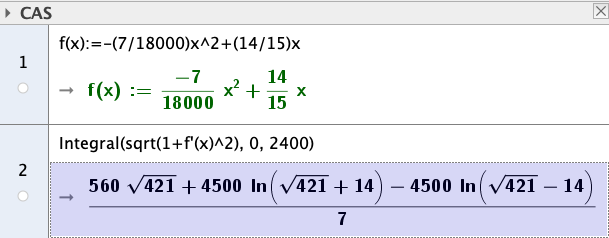
\includegraphics[scale=0.7]{CAS.png}
\end{center}
\caption{Integralet løst med CAS}
\label{fig:CAS}
\end{figure}

\end{document}
